\chapter{Design of the Envoy File System}

This chapter examines the storage needs of service clusters and how they can be accommodated. Service clusters place specific demands on the storage system to efficiently support the deployment and management of untrusted services, but they also present helpful properties that can simplify the job. In addition to detailing these constraints, this chapter describes Envoy, a file system designed for this environment.

\section{Design goals and principles}

\subsection{Things that a service cluster calls for}
\begin{itemize}
\item exploit admin domain for simple security and fault model
\item expect lots of redundancy in disk images; aggregate cache
\item support mobile VMs
\item support rapid deployment of services with lightweight file system forks
\item use cheap commodity disks
\item snapshots
\item isolate services from each other, but allow cooperative groups
\end{itemize}

\subsection{Desirable properties that the envoy model achieves}
\begin{itemize}
\item distribute only when there's a reason; favor centralization when practical
\item perfectly consistent persistent caching
\item local impact---heavy users bear most of the load, non-users none of it
\item serve from local machine cache when uncontended, NFS-like when shared: requests never require topology changes
\item in steady state, coordination based on actual contention, not potential contention
\item simple security model that maps well to familiar Unix semantics
\item private images act like local images, shared images scale gracefully
\end{itemize}

\section{Using Envoy}

\subsection{Basic environment and assumptions}


It's a cluster, dom0 is trusted, it's all managed together, expect users to start from standard installs

\subsection{Use and administration}

This section presents the administrative interface to Envoy, which is designed as a series of special file operations and conventions.

All services share a single cluster-wide namespace tree with a common root. Mounting the root of the entire tree requires special priviledges, normally reserved for the administrative tools managing the file system. The top levels of the hierachy respond normally to standard file operations, with a few notable exceptions described here.

A few file names are given special significance and their use is restricted. The name \current is reserved for use as the root of a client file system, positive integers are reserved as the read-only roots of snapshots (in ascending order) of the tree rooted at \current in the same directory, and a symbolic link names \snapshot is created and protected by the system to link to the most recently-created snapshot in the same directory. In addition, a normal file named \password can exist to store credentials for clients accessing descendents of the containing directory.

The namespace is conceptually divided between the administrative levels and the client levels. The client levels include anything that is a descendent of a directory named \current or one of its snapshots (named as positive integers). Any path that does not pass through one of these points is considered part of the administrative namespace and is subject to the restrictions and special semantics described in this section.

To create a new file system root, a user or management tool creates any desired layers of files and directories within the administrative area, ending with a directory called \current. Services can then mount \current or any of its descendent directories. A client mount request specifies the desired root pathname along with the username attempting the mount and any credentials required to validate the request. The server checks these credentials against any files called \password that it encounters in administrative directories passed through before arriving at \current, with those further down the hierarchy overriding those encountered earlier.

In addition to end-user mounts, this system of password files applies to the administrative file areas as well. If given suitable credentials, a service can attach to the namespace in an administrative directory to create and manage its own file system trees and credential files, creating a hierachy for management roles as well as file storage. Controlling access to any directory requires credentials to mount its parent, along with standard file permissions within the parent directory to manipulate the credential file. Envoy does not map user and group names to numeric IDs, so any clients that can agree on usernames and credentials can share access to a file system.

In addition to marking the transition from administrative to client directories, a directory named \current can have its snapshot taken. When the server receives a request to create a symbolic link with a positive integer as its name and \current as its target, it checks to make sure that the integer is correct for the next snapshot (either \texttt{1} or the number linked to by \snapshot plus one). If so, it takes a snapshot of \current, makes it accessible using the requested name (accessible as a directory, not a symbolic link), and creates or updates \snapshot to link to the newly created snapshot. Any request with the wrong target or the wrong number is rejected.

Snapshots are always given positive integers as names (and cannot be renamed), but this is not always convenient for use. It may be useful to name a particular snapshot with a more meaningful name using a symbolic link. Symbolic links are normally considered opaque by the server and cannot be used in any mount or directory-change requests, so to make accessing named snapshots more convenient the server silently dereferences symbolic links that refer to snapshots in the same directory.

Snapshots also serve another special purpose: they can be used as the root for a file system fork operation. Just as the \current directory diverges from its most recent snapshot using copy-on-write semantics, new \current roots in other administrative directories can use an existing snapshot as a starting point. A request to create a symbolic link called \current that refers to the fully-qualified pathname of a snapshot (again, links to a snapshot within the same directory are dereferenced, but others are not) is treated as a fork operation using the given snapshot as the starting point for a new root file system. The newly forked file system is subject to the same rules as those created with \texttt{mkdir}, and respects the credentials local to its creation site, not those of the snapshot from which it diverges. For this reason, fork operations require sufficient credentials at both locations.

\section{Architecture}

Services access Envoy using a client-server network file system interface. Each physical machine in the service cluster runs an administrative virtual machine that manages the storage processes for all services on that machine. The services on this VM partition the local disk between a constribution to the shared storage pool and the local persistent cache as well as providing a standard interface allowing other hosts on the machine to access the file system. Figure~\ref{fig:single-machine} illustrates a typical machine.

\begin{figure}[tp]
\centering
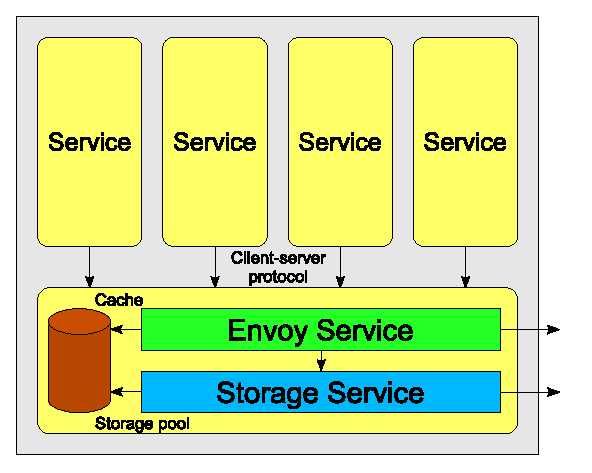
\includegraphics{figures/single-machine}
\caption{Each physical machine has a single administrative VM that hosts the Envoy services. This VM exports a network file system protocol to other service VMs running on the same machine.}
\label{fig:single-machine}
\end{figure}

The file system management processes join a cluster-wide service that is comprised of two primary layers, as illustrated in Figure~\ref{fig:layers}. Storage is managed by the lower level, which allows a small set of basic file operations on objects. All operations are stateless and the storage service makes no attempt to prevent or manage concurrent requests or to enforce any kind of security policy. Objects are extents of bytes with a small set of attributes.

On top of the storage service is the Envoy layer, which builds a hierarchical file system out of objects, coordinates access to files, provides authentication and access control services, manages caching, and exports a standard network file system interface for services to access.

\begin{figure}[tp]
\centering
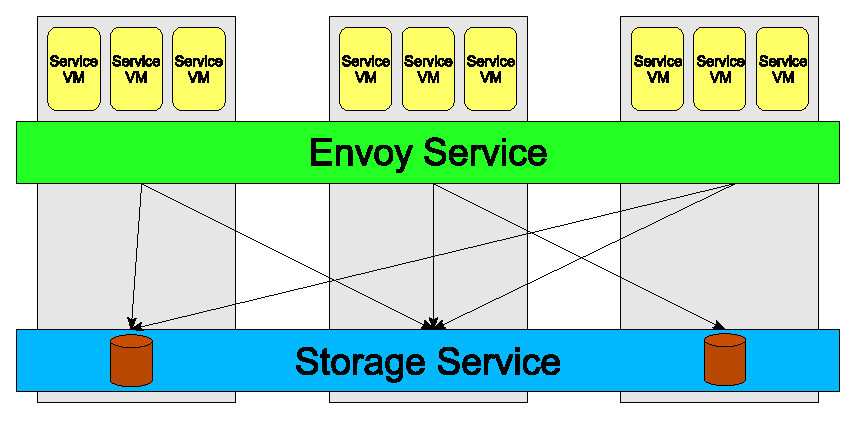
\includegraphics{figures/layers}
\caption{The Envoy services coordinate access to provide a single, coherent view of the distributed file system. It relies on the storage service, which provides a repository of objects referenced by unique identifiers.}
\label{fig:layers}
\end{figure}

In the remainder of this section I detail the functionality and requirements of these systems and consider the tradeoffs of various design decisions.

\subsection{Distribution}

Envoy is designed to run in a trusted environment with direct access to the local disk.

\subsection{Storage layer}

The abstractions to provide redundancy and data distribution are encapsulated in the storage layer. The storage layer provides a simple interface supporting a few basic operations on objects that are referenced by unique identifiers. Objects can be created, deleted, and cloned, byte ranges within objects can be read from and written to, and the attributes of objects can be queried and modified.

Object managements services have grown in popularity in recent years. They offer a simple mapping from files and directories to the underlying mechanism that makes the overall system easier to comprehend and design, as well as implement, debug, and maintain.

This seperation is also a convenient way to divide lower-level storage concerns such as reliability and availability from higher-level file system responsibilities, including consistency, security, cache policy, and conflict resolution.

\subsection{Envoy layer}
\subsubsection{Data layout}

\subsection{Caching}
\subsubsection{Data paths for typical requests}

\section{Operations}
\subsection{File operations and state management}
\subsection{Forks and snapshots}
\subsection{Lease migration}
\subsection{Security}
\subsection{Deleting snapshots}

\section{Recovery}

\section{Summary}